\section{Thursday}\index{Thursday_lecture}
\subsection{$\second$ order Quasi-linear}
\[a\uxx+2b\uxy+c\uyy=d
\]
$a$, $b$, $c$, $d$ are functions of $(x,y,u,\ux,\uy)$\\
Initial curve $f(s)$, $g(s)$. Initial value $u=h(s),\ux=\varphi(s), \uy=\psi(s)$.\\
\[u(f(s),g(s))=h(s)
\]
\[\ux f\p+\uy g\p=h\p
\]
\[\varphi f\p+\psi g\p=h\p
\]
Assume the above equation is satisfied.
\[\ux(f(s),g(s))=\varphi(s)\qquad\uy(f(s),g(s))=\psi(s)
\]
\[\uxx f\p+\uxy g\p=\varphi \p\qquad u_{yx}f\p+\uyy g\p=\psi\p
\]
\[\begin{pmatrix}a&2b&c\\f\p&g\p&0\\0&f\p&g\p\end{pmatrix}\begin{pmatrix}\uxx\\\uxy\\\uyy\end{pmatrix}=\begin{pmatrix}d\\\varphi\p\\\psi\p\end{pmatrix}
\]
\[0=\begin{vmatrix}a&2b&c\\f\p&g\p&0\\0&f\p&g\p\end{vmatrix}=a{g\p}^2-2bf\p g\p+c{f\p}^2
\]
Personal understanding (may not be correct):\\
This is called characteristic curve for when determinant is equal to zero above system will not have a solution. This situation will on happen when the initial curve $(f,g,h)$is tangent to a charateristic curve at every point. Therefore, $a{g\p}^2-2bf\p g\p+c{f\p}^2$.
\[\dakuohao{x=f(s)}{y=g(s)}\quad\dakuohao{\deriv{x}{s}=f\p}{\deriv{y}{s}=g\p}~\Rightarrow~\deriv{y}{x}=\frac{g\p}{f\p}
\]
\[a(\deriv{y}{x})^2-2b\deriv{y}{x}+c=0
\]
\[\deriv{y}{x}=\frac{2b\pm\sqrt{2b^2-4ac}}{2a}
\]
\begin{itemize}
\item $b^2-ac>0$: Hyperbolic
\item $b^2-ac=0$: Parabolic
\item $b^2-ac<0$: Elliptic

\end{itemize}
\begin{example}

\begin{itemize}
\item $\uyy-c^2\uxx=0$ $A=-c^2, B=0, C=1\Rightarrow~B^2-AC=C^2$
\item heat equation $\uy=c^2=\uxx=0$  $A=-C^2, B=0, C=0~\Rightarrow~B^2-AC=0$
\item laplace equation $\uyy+\uxx=0$ $A=1=C, B=0~\Rightarrow~B^2-AC=-1<0$
\end{itemize}
\end{example}

Wave equation
\[\uyy-c^2\uxx=0
\]
\[\deriv{y}{x}=\frac{1}{-c^2}(\pm c)=\mp\frac{1}{c}
\]
\[y=\mp\frac{1}{c}x+\text{const}
\]
\[y\pm\frac{1}{c}x=\text{const}
\]
\[\xi=y+\frac{1}{c}x
\]
\[\eta=y-\frac{1}{c}x
\]
\[v(\xi,\eta)=u(x(\xi,\eta),y(\xi,\eta))
\]
\[u(x,y)=v(\xi(x,y),\eta(x,y))
\]
\[\ux=v_{\xi}\xi_{x}+v_\eta\eta_x=v_{\xi}\frac{1}{c}-v_\eta\frac{1}{c}
\]
\[\uxx=v_{\xi\xi}\frac{1}{c^2}+v_{\xi\eta}(-\frac{1}{c^2})-v_{\eta\xi}\frac{1}{c^2}+v_{\eta\eta}\frac{1}{c^2}
\]
\[\uy=v_\xi\xi_y+v_\eta\eta_y=v_\xi+v_\eta
\]
\[\uyy=v_{\xi\xi}+2v_{\xi\eta}+v_{yy}
\]
\[0=\uyy-c^2\uxx=v_{\xi\xi}+2v_{\xi\eta}+v_{yy}-v_{\xi\xi}+2v_{\xi\eta}-v_{\eta\eta}=4v_{\xi\eta}
\]
\[v_{\eta\xi}=0~\Rightarrow~(v_\xi)_\eta=0~\Rightarrow ~v_\xi=f\p(\xi)
\]
\[v=f(\xi)=\text{const in }\xi
\]
\[v(\xi,\eta)=f(\xi)+g(\eta)=u(x,y)=f(y+\frac{1}{c}x)+g(y-\frac{1}{c}x)
\]
An observation:
\[u(A)+u(C)=f(y_A+\frac{1}{c}x_A)+g(\underline{\red y_A-\frac{1}{c}x_A})+f(y_C\frac{1}{c}x_C)+g(y_C-\frac{1}{c}x_C)
\]
\[u(B)+u(D)=f(y_B+\frac{1}{c}x_B)+g(\underline{\red y_B-\frac{1}{c}x_B})+f(y_D\frac{1}{c}x_D)+g(y_D-\frac{1}{c}x_D)
\]
\begin{figure}[H]
\centering
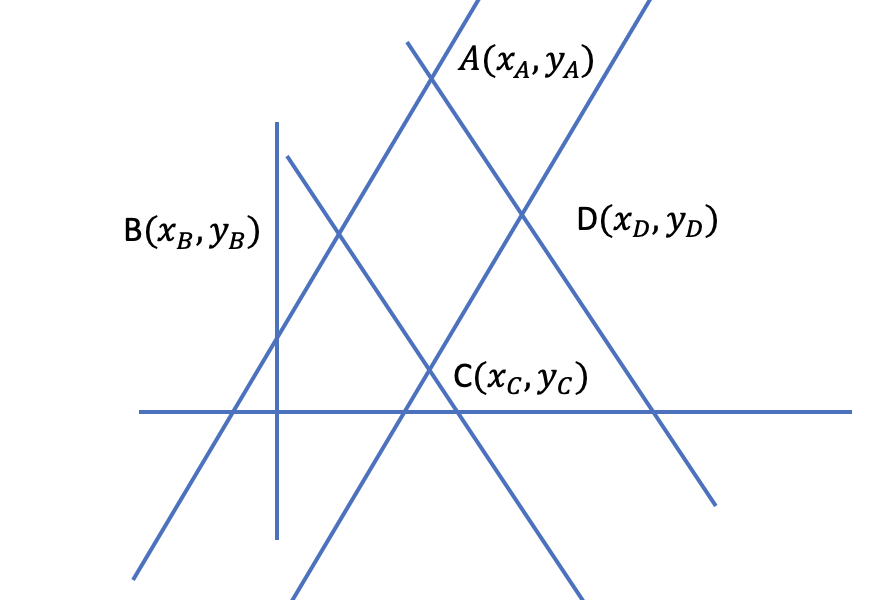
\includegraphics[width=8cm]{w2_th1}
\end{figure}
Take $c=1$ for simplicity
\[\left\{\begin{gathered}\uyy-\uxx=0\\u(x,0)=\varphi(x)\\\uy(x,0)=\psi(x)\end{gathered}\right.
\]
\[u(x,y)=f(y+x)+g(y-x)
\]
\[\varphi(x)=u(x,0)=f(x)+g(-x)
\]
\[\psi(x)=\uy(x,0)=f\p(x)+g\p(-x)
\]
\[\varphi(x)=f(x)+g(-x)~\Rightarrow~\varphi\p(x)=f\p(x)-g\p(-x)
\]
\[\dakuohao{\varphi(x)=f(x)=g(-x)}{\psi(x)=f\p(x)=g\p(x)}\Rightarrow \psi\p(x)=f\p(x)-g\p(-x)
\]
\[\frac{\varphi\p(x)+\psi(x)}{2}=f\p(x)\Rightarrow~f(x)=\frac{1}{2}\psi(x)+\frac{1}{2}\int_0^x\psi(s)\diff s+\text{const}\alpha
\]
\[\frac{-\varphi\p(x)+\psi(x)}{2}=g\p(-x)~\Rightarrow~g(-x)=\frac{1}{2}\varphi(x)-\frac{1}{2}\int_0^x\psi(s)\diff s+\text{const}\beta
\]
\[\begin{aligned}u(x,y)&=f(x+y)+g(y-x)\\&=\frac{1}{2}\varphi(x+y)+\frac{1}{2}\int_0^{x+y}\psi(s)\diff s+\alpha+\frac{1}{2}\varphi(x-y)-\frac{1}{2}\int_0^{x-y}\psi(s)\diff s+\beta\\&=\frac{1}{2}[\varphi(x+y)+\varphi(x-y)]+\frac{1}{2}\int_{x-y}^{x+y}\psi(s)\diff s+\alpha+\beta\end{aligned}
\]
\\
\[u(x,y)=\frac{1}{2}[\varphi(x+y)+\varphi(x-y)]+\frac{1}{2}\int_{x-y}^{x+y}\psi(s)\diff s
\]
\[\begin{cases}\uyy-\uxx=0\\u(x,0)=\varphi(x)\text{--initial displacement}\\\uy(x,0)=\psi(x)\text{--initial velocity}\end{cases}
\]
case(i) $\psi\equiv0$ $t=y=1$ $u(x,1)=\frac{1}{2}\varphi(x+1)+\frac{1}{2}\varphi(x-1)$
\begin{figure}[H]
\centering
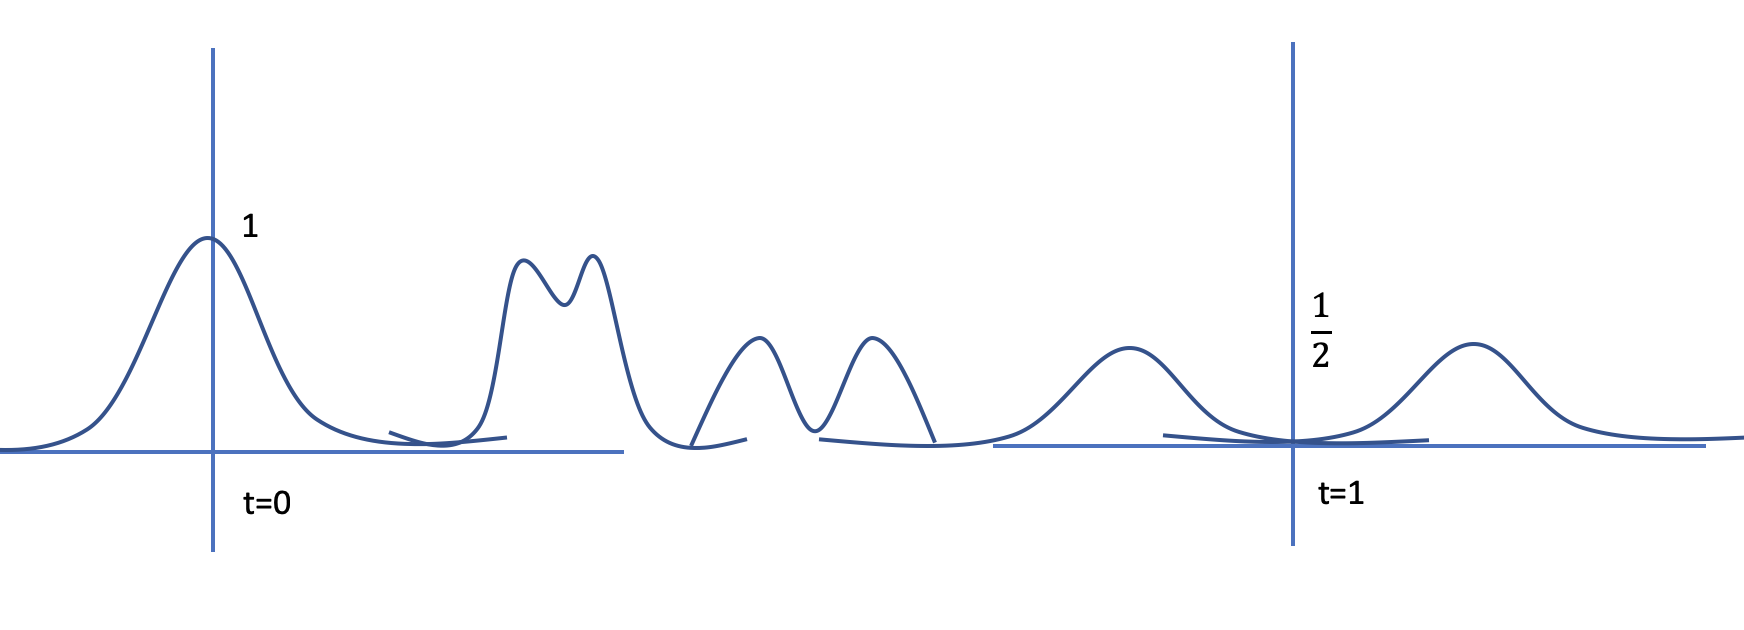
\includegraphics[width=12cm]{w2_th2}
\end{figure}
case(ii)$\psi=0$
\begin{figure}[H]
\centering
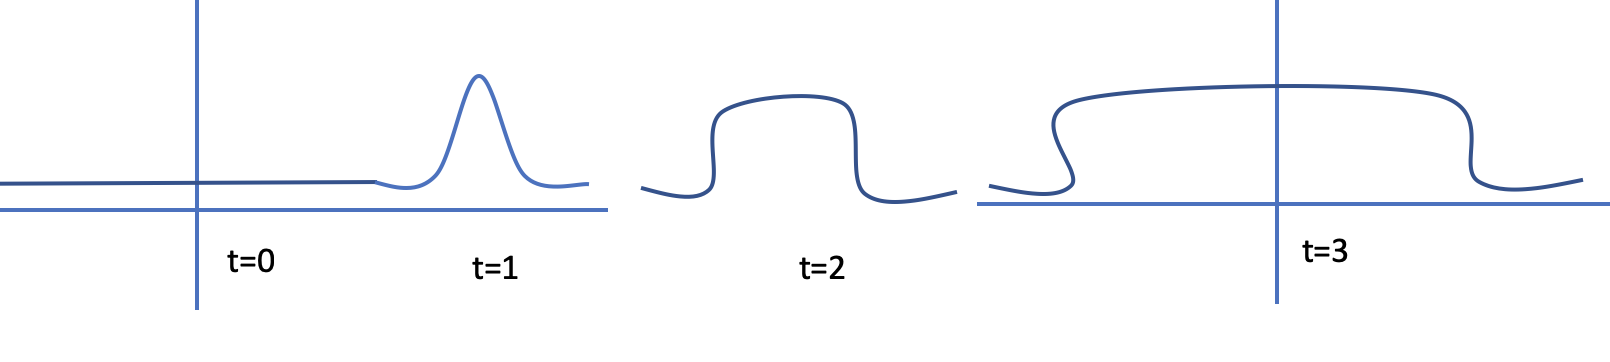
\includegraphics[width=13cm]{w2_th3}
\end{figure}